\section{Provable Security Analysis of Privacy}
\label{sec:privacy}


In this section, we will give the proof that UPPRESSO is defensive to both IdP-based login tracing and RP-based identity linkage, based on DDH assumption\cite{GoldwasserK16}, the computational problem. 


\noindent\textbf{DDH Assumption.}
$\mathbb{G}$ is a q-order  cyclic additive group of $E(\mathbb{F}_p)$, where $q$ and $n$ are large primitive number, and $P$ is the generator of $\mathbb{G}$.  For any PPT algorithm $D$, the distributions, \{$P$, $aP$, $bP$, $abP$\}$_{a,b \in \mathbb{Z}_n}$ and \{$P$, $aP$, $bP$, $cP$\}$_{a,b,c \in \mathbb{Z}_n}$, are computationally indistinguishable. There is a negligible $\sigma(k)$, where $k$ is the security parameter. 
\begin{multline*}
    \ \ \ \ \ \ \ Pr[D(P, aP, bP, abP)=1]\\-Pr[D(P, aP, bP, cP)=1]=\sigma(k)\ \ \ \ \ \ \ \ 
\end{multline*}

\noindent\textbf{IdP-based identity linkage.} 
It can be found in figure~\ref{fig:process} that the only parameter related with RP's identity and received by IdP is $PID_{RP}$. Moreover, $PID_{RP}$ is created based on $ID_{RP}$ and the IdP uncontrolled random number $N_U$. As $N_U$ is randomly chosen in $\mathbb{Z}_n$,  $PID_{RP}$ is also the randomly chosen point in $\mathbb{G}$ to IdP. Therefore, obviously IdP cannot trace the user's login RPs, so that IdP-based identity linkage is not possible in UPPRESSO.

\noindent\textbf{RP-based identity linkage.} 
\begin{figure}[t]
  \centering
  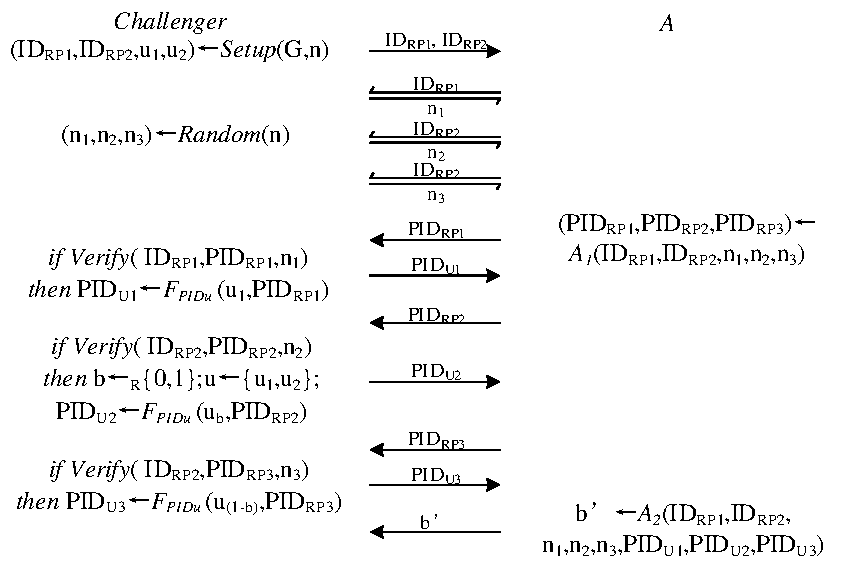
\includegraphics[width=1\linewidth]{fig/game0.pdf}
  \caption{Game0.}
  \label{fig:game0}
\end{figure}
In the \emph{RP-based identity linkage} scenario, collusive RPs conduct the malicious behavior against IdP and users to relate the user in different RPs. It can be considered as a $Game$ guessing whether $PID_U$s for different RPs belong to the same user.  In this $Game$ IdP and users act as the challenger, and RPs act as the adversary. 

\textbf{If only it can be proved that the adversary cannot take any advantage of guessing whether $PID_U$s belong to same $ID_U$, RP-based identity linkage should be considered impossible in UPPRESSO.}

Firstly we give the realistic model of the $ID_U -guessing- Game$, shown as figure~\ref{fig:game0}. While $b=b'$ is true, we consider the adversary succeed.
We define the event [$b'=b$] in Game 0 as $\Gamma$. The probability $Pr[\Gamma]$ must be 1/2 as if  the adversary cannot take any advantage of guessing $b$ (i.e.  whether $PID_U$s belong to same $ID_U$). Therefore, it is proved that UPPRESSO is protected from RP-based identity linkage as $Pr[\Gamma]=1/2$.

Then we build the ideal model of Game, of which the probability  that an adversary succeeds to guessing $b$ is 1/2. The model is shown as figure~\ref{fig:game1}. As $z$ and $r$ is randomly generated and unknown to $A$, the adversary has no information about $b$. We  define the event [$b'=b$] in Game 1 as $\Gamma_1$. $Pr[\Gamma_1]$ must be equal to 1/2. 

Therefore, we only need to prove that $|Pr[\Gamma_1]-Pr[\Gamma]|=\sigma(n)$, where $\sigma(n)$ is negligible. Here we give another model of Game 2, shown as figure~\ref{fig:game2}. We can find that in fact it only sets the exact values of the parameters defined in Game 0, such as $ID_{RP2}=xID_{RP1}$, $u_1=y$ and $u_2=r$(r is a random number).  Here we define the event [$b'=b$] in Game 2 as $\Gamma_2$. There should be $Pr[\Gamma_2]=Pr[\Gamma]$.

We are going to prove that $|Pr[\Gamma_1]-Pr[\Gamma_2]|=\sigma(n)$

\begin{figure}[t]
  \centering
  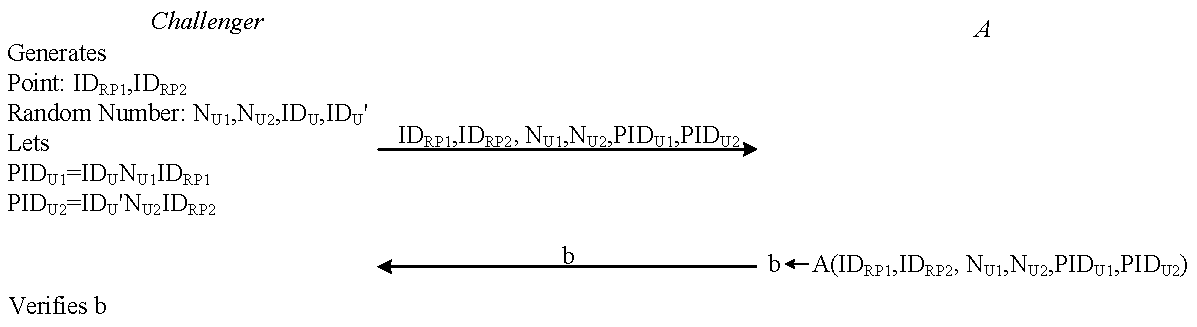
\includegraphics[width=1\linewidth]{fig/game1.pdf}
  \caption{Game1.}
  \label{fig:game1}
\end{figure}




\begin{figure}[t]
  \centering
  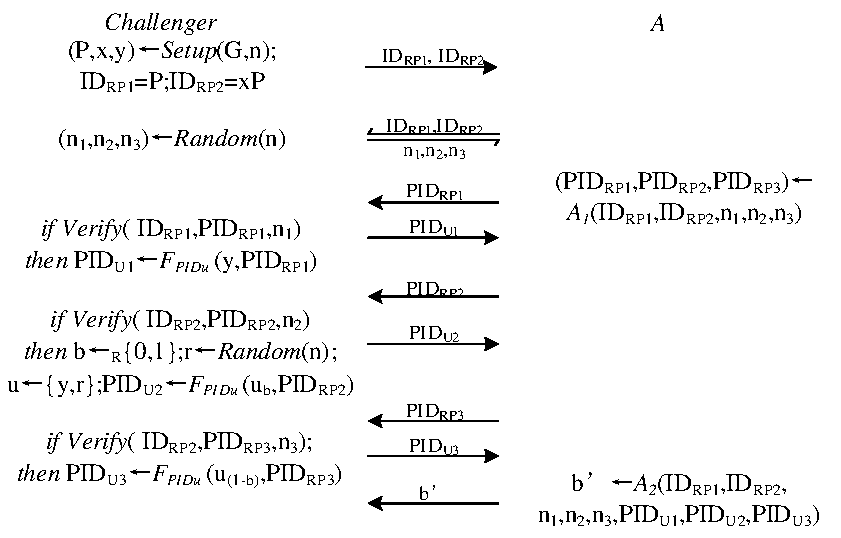
\includegraphics[width=1\linewidth]{fig/game2.pdf}
  \caption{Game2.}
  \label{fig:game2}
\end{figure}